 \documentclass[a4paper,10pt]{article}
\usepackage{marvosym}
\usepackage{fontspec} 					
\usepackage{xunicode,xltxtra,url,parskip} 	
\RequirePackage{color}
\usepackage[usenames,dvipsnames]{xcolor}
\usepackage[big]{layaureo} 			
\usepackage{supertabular} 			
\usepackage{titlesec}
\usepackage{hyperref}
\usepackage{graphicx}
\graphicspath{ {images/} }
\definecolor{linkcolour}{rgb}{0.4,0.4,0.6}
\hypersetup{colorlinks,breaklinks,urlcolor=linkcolour, linkcolor=linkcolour}

\defaultfontfeatures{Mapping=tex-text}
%\setmainfont[SmallCapsFont = Fontin SmallCaps]{Fontin}
%%% modified for Karol Kozioł for ShareLaTeX use
\setmainfont[
SmallCapsFont = Fontin-SmallCaps.otf,
BoldFont = Fontin-Bold.otf,
ItalicFont = Fontin-Italic.otf
]
{Fontin.otf}


\titleformat{\section}{\Large\scshape\raggedright}{}{0em}{}[\titlerule]
\titlespacing{\section}{0pt}{10pt}{3pt}
%Tweak a bit the top margin
%\addtolength{\voffset}{-1.3cm}

%Italian hyphenation for the word: ''corporations''
\hyphenation{im-pre-se}

%-------------WATERMARK TEST [**not part of a CV**]---------------
\usepackage[absolute]{textpos}

\setlength{\TPHorizModule}{30mm}
\setlength{\TPVertModule}{\TPHorizModule}
\textblockorigin{2mm}{0.65\paperheight}
\setlength{\parindent}{0pt}
%--------------------BEGIN DOCUMENT----------------------
\begin{document}

%WATERMARK TEST [**not part of a CV**]---------------
%\font\wm=''Baskerville:color=787878'' at 8pt
%\font\wmweb=''Baskerville:color=FF1493'' at 8pt
%{\wm 
%	\begin{textblock}{1}(0,0)
%		\rotatebox{-90}{\parbox{500mm}{
%			Typeset by Alessandro Plasmati with \XeTeX\  \today\ for 
%			{\wmweb \href{http://www.aleplasmati.comuv.com}{aleplasmati.comuv.com}}
%		}
%	}
%	\end{textblock}
%}

\pagestyle{empty} % non-numbered pages

\font\fb=''[cmr10]'' %for use with \LaTeX command

%--------------------TITLE-------------
% \hrulefill
\par{\filleft
		{\Large \textsc{Swati Gavas}
		\\
% 		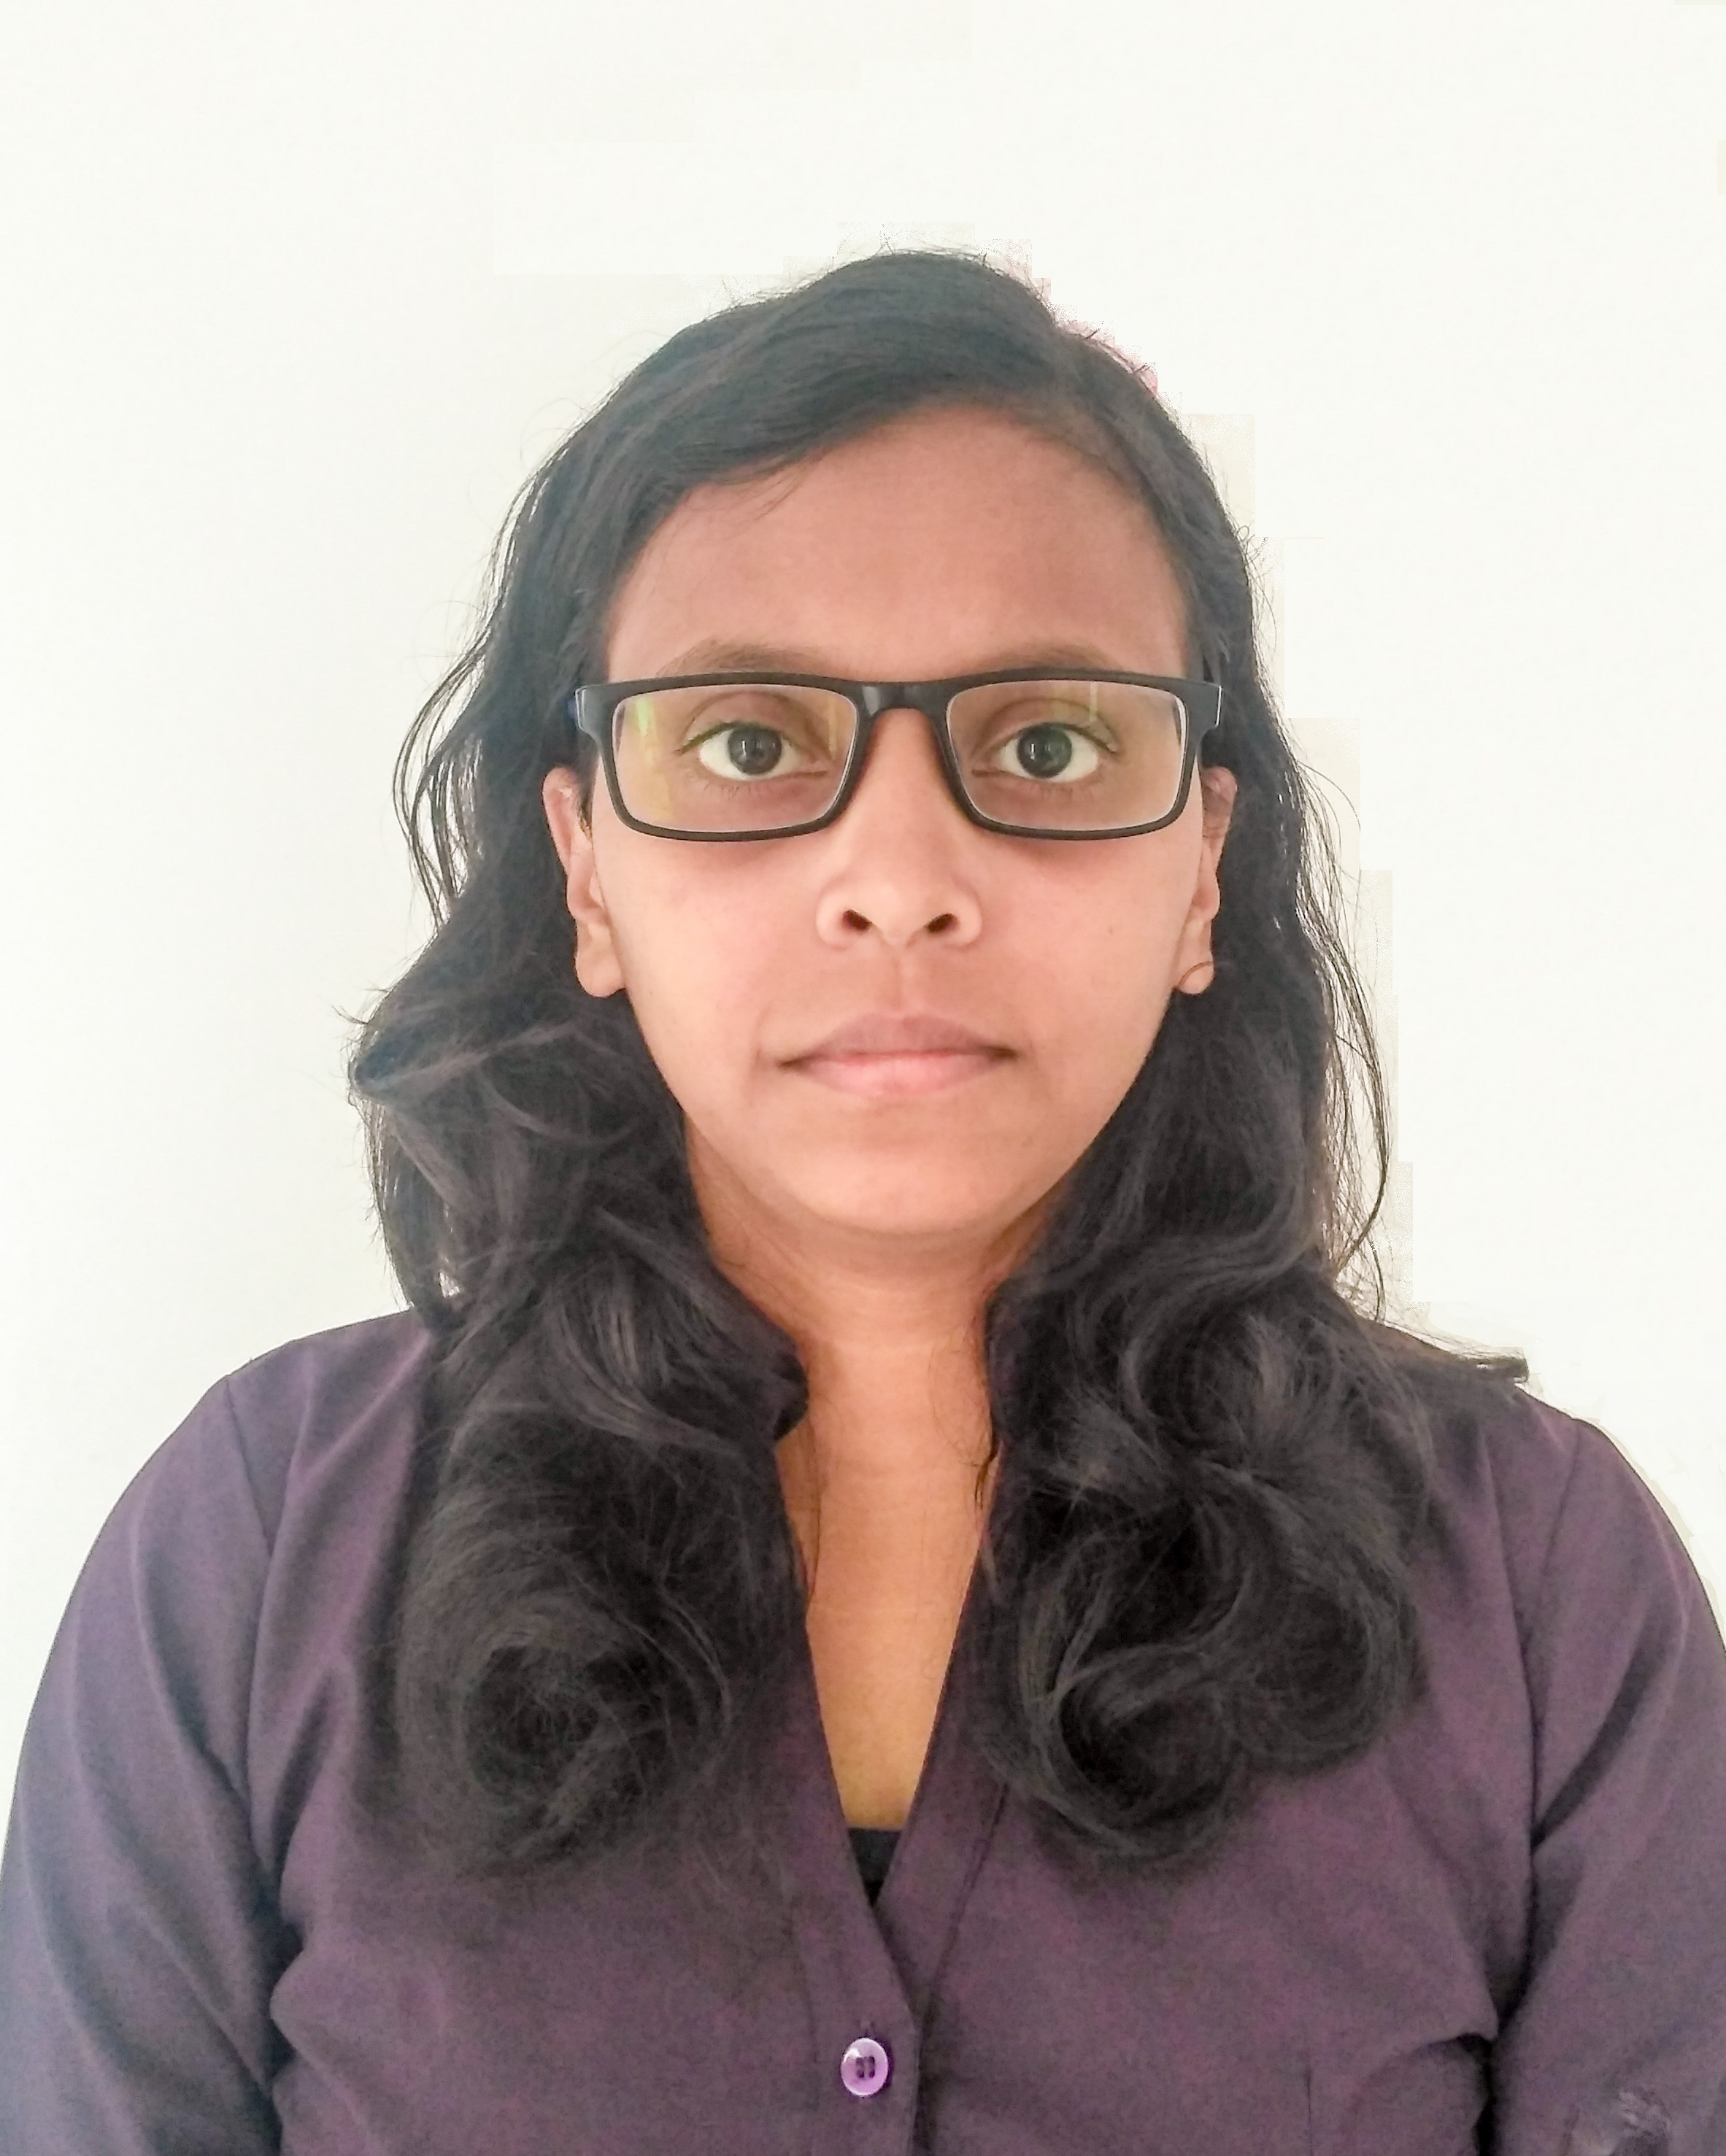
\includegraphics[scale=0.035]{photo.jpg}
	}\par}
\vspace{0.2cm}
% \hrulefill

%--------------------SECTIONS-----------------------------------
%Section: Personal Data
\section{Personal Data}

\begin{tabular}{rl}
    \textsc{Place and Date of Birth:} & Kolhapur, Maharashtra, India  | July 1994 \\
     \textsc{Nationality and Gender:} & Indian  | Female \\
      \textsc{Webpage:} & \href{https://swati-gavas.github.io/profile/}{swati-gavas.github.io/profile/} \\
    % \textsc{Address:}   & A/P - Isapur, Chandgad, Kolhapur, MH, India- 416509 \\
    \textsc{Phone and email:}     & +91 70XXXXXX64 | \href{mailto:swatigavas47@gmail.com}{swatigavas47@gmail.com}\\
    % \textsc{Phone and email:}     & +91 7021983364 | \href{mailto:swati.s.gavas@gmail.com}{swati.s.gavas@gmail.com}\\
    % \textsc{email:}     &   \href{mailto:swati.s.gavas@gmail.com}{swati.s.gavas@gmail.com}
\end{tabular}

\section{Post-Doctoral Positions}
\begin{tabular}{rl}
    \textsc{Tenure:} & July 2026 - present \\
    \textsc{Advisor/Host:}   & \href{https://gax.sjtu.edu.cn/jxhan/node/4}{Dr. Jiaxin Han} \\
    \textsc{Institute:}     & Shanghai Jiao Tong University, Shanghai\\ \\

    \textsc{Tenure:} & APR 2025 - MAR 2026 \\
    \textsc{Advisor/Host:}   & \href{https://niser.irins.org/profile/241972}{Dr. Nishikanta Khandai} \\
    \textsc{Institute:}     & National Institute of Science Education and Research (NISER), Bhubaneswar\\
\end{tabular}


%Section: PhD
\section{PhD}

\begin{tabular}{rl}
    \textsc{Tenure:} & AUG 2018 - DEC 2024 \\
    \textsc{Topic:} & Aspects of gravitational clustering and structure formation in the Universe \\
    \textsc{Advisor:}   & \href{https://web.iisermohali.ac.in/Faculty/jasjeet/index.html}{Prof. Jasjeet Singh Bagla}
    % , \href{https://niser.irins.org/profile/241972}{Dr. Nishikanta Khandai}
    \\
    \textsc{Institute :}     & Indian Institute of Science Education and Research (IISER), Mohali\\
\end{tabular}

%Section: Education
\section{Education}
\begin{tabular}{rl}	
\textsc{July} 2017 & Master of Science in \textsc{Physics}, \\ &\textbf{Department of Physics, Savitribai Phule Pune University}, Pune\\
& Major: Astronomy and Astrophysics | \normalsize \textsc{Cgpa}: 8.27/10 \\&\\

\textsc{July} 2015& Bachelor of Science in \textsc{Physics} \\& DBJ College, Chiplun, \normalsize\textbf{Mumbai University} | \normalsize \textsc{Cgpa}: 7/7 
\\& Secured third rank at the University level\\&\\

\textsc{Apr} 2012& Higher Secondary Certificate\\
& DBJ College, Chiplun, \textbf{Maharashtra State Board} | \textsc{Percentage}: 88.17\% \\&\\

\textsc{Apr} 2010& Secondary School Certificate\\
& Alore High school, Chiplun, \textbf{Maharashtra State Board} | \textsc{Percentage}: 94.18\% \\
\end{tabular}

%Section: PhD
\section{Research Interest}
\begin{itemize}
    \item Gravitational clustering and large-scale structure formation through cosmological simulations and analytical modeling, linking theory with survey observations.
    \item Dark matter halos, galaxy formation, and baryonic processes
    % \item Thermodynamics of late-time cosmology
\end{itemize}

%Section: Publications
\section{Publications \href{https://tinyurl.com/2vhkj2m6}{\small{NASA-ADS}}}

\begin{tabular}{rl}
    \textsc{2022 :} & Swati Gavas, Jasjeet Bagla, Nishikanta Khandai, Girish Kulkarni\\ & Halo mass function in scale invariant models,\\& \href{https://doi.org/10.1093/mnras/stad935}{MNRAS, Volume 521, Issue 4, June 2023, Pages 5960–5971}   \\
\end{tabular}

\begin{tabular}{rl}
    \textsc{2024 :} & Swati Gavas, Jasjeet Bagla, Nishikanta Khandai\\ & Dispersion in the Hubble-Lema\^itre constant measurements from \\ & gravitational clustering,\\ & \href{https://journals.aps.org/prd/abstract/10.1103/PhysRevD.111.043516}{Phys. Rev. D 111, 043516 – 10 February, 2025}   \\
\\
 & Jasjeet Bagla, Swati Gavas\\ & On the origin of transient features in cosmological N-Body Simulations,\\ &\href{https://link.springer.com/article/10.1007/s12036-025-10055-x}{JOAA, Volume 46, article number 33, 16 June 2025}   \\
\end{tabular}

\begin{tabular}{rl}
    \textsc{2025 :} & Dipayan Mukherjee, Harkirat Singh Sahota, Swati Gavas\\ & A dynamical systems perspective on the thermodynamics of late-time cosmology\\&
    \href{https://onlinelibrary.wiley.com/doi/10.1002/prop.70094}{Fortschritte der Physik, VL:74, IS:4, SN:0015-8208}\\
\end{tabular}

\begin{tabular}{rl}
    \textsc{2026 :}
 & Ayan Nanda, Nishikanta Khandai, Jasjeet Singh Bagla, Swati Gavas\\ & Universality of Halo Shape and its Morphological Evolution across Cosmic Time.\\ &
 \href{https://arxiv.org/abs/2603.26640}{astro.ph-CO}\\
\\
& [In preparation]\\ & Swati Gavas, Ayan Nanda, Nishikanta Khandai\\ & Finite box size effect on halo scales\\ %&\href{}{astro-ph.CO }   \\
\\
& [In preparation]\\ & {Ayan Nanda, Nishikanta Khandai, Swati Gavas}\\ & Multipole Characterization of Triaxial Dark Matter Halos:\\& A Spherical Harmonic Approach\\ %&\href{}{astro-ph.CO }   \\
\end{tabular}


\section{conferences, Schools and Workshops}

\begin{tabular}{p{2.5cm} p{11cm}}

\textsc{29-2 Oct 2025:} & {(presented talk)}\\ 
& \textbf{{Challenges and Innovations in Computational Astrophysics VI} }\\
& \footnotesize{Held at Indian Institute of Science Education and Research (IISER), Mohali}\\
& \footnotesize{Talk title: Numerical Artifacts of Restricted Power Spectrum in cosmological N-Body Simulations}\\ \\
\end{tabular}

\begin{tabular}{p{2.5cm} p{11cm}}

\textsc{11 Nov 2024:} & {(presented talk)}\\ 
& \textbf{{Computational and Observational Cosmology Group at the Observat\'orio Nacional - ON(RJ/Brazil)} }\\
& \footnotesize{Talk title: Dispersion in the Hubble-Lema\^itre constant measurements from gravitational clustering}\\ \\
\end{tabular}


\begin{tabular}{p{2.5cm} p{11cm}}
\textsc{14-25 Oct 2024:} & \textbf{{3rd IAGRG School on Gravitation and Cosmology} }\\
& \footnotesize{Held at International Centre for Theoretical Sciences (ICTS), Bengaluru, India}\\ \\
\end{tabular}

\begin{tabular}{p{2.5cm} p{11cm}}
\textsc{1-2 July 2024:} & {(presented talk)}\\ 
& \textbf{{S\'eminaire Univers Institut d'Astrophysique de Paris (IAP)} }\\
& \footnotesize{Visit to Prof. Stephane Colombi at Institut d'Astrophysique de Paris (IAP), France}\\
& \footnotesize{Talk title: Halo mass function in scale-invariant models}\\ \\

\end{tabular}
\begin{tabular}{p{2.5cm} p{11cm}}

\textsc{17-28 June 2024:} & {(presented talk)}\\ 
& \textbf{{Summer School on Cosmology} }\\
& \footnotesize{Held at International Centre for Theoretical Physics (ICTP), Trieste, Italy}\\
& \footnotesize{Talk title: Dispersion in the Hubble-Lema\^itre constant measurements from gravitational clustering}\\ \\
\end{tabular}
\begin{tabular}{p{2.5cm} p{11cm}}

\textsc{1-4 Feb 2024:} & {(presented talk)}\\ 
& \textbf{{42nd Meeting of Astronomical Society of India} }\\
& \footnotesize{Held at IISc, ISRO and JNP Bengaluru, India}\\
& \footnotesize{Talk title: Dispersion in the Hubble-Lema\^itre constant measurements from gravitational clustering}\\ \\
\end{tabular}
\begin{tabular}{p{2.5cm} p{11cm}}

\textsc{6-9 Dec 2023:} & {(presented talk)}\\ 
& \textbf{{10th International Conference on Gravitation and Cosmology} }\\
& \footnotesize{Held at IIT Guwahati, India}\\
& \footnotesize{Talk title: A Local Perspective on Hubble Tension from Cosmological N-body Simulations}\\ \\
\end{tabular}
\begin{tabular}{p{2.5cm} p{11cm}}

\textsc{7-9 Nov 2023:} & {(presented talk)}\\ 
& \textbf{{Challenges and Innovations in Computational Astrophysics V} }\\
& \footnotesize{Virtual Meeting}\\
& \footnotesize{Talk title: A Local Perspective on Hubble Tension from Cosmological N-body Simulations}\\ \\
\end{tabular}
\begin{tabular}{p{2.5cm} p{11cm}}

\textsc{24-28 Oct 2022:} & {(presented talk)}\\ 
& \textbf{{The 10th KIAS Workshop on Cosmology and Structure Formation} }\\
& \footnotesize{Held at KIAS, South Korea}\\
& \footnotesize{Talk title : Halo mass function in scale invariant models}\\ \\
\end{tabular}

\begin{tabular}{p{2.5cm} p{11cm}}
\textsc{2-6 Nov 2020:} & {(presented poster talk)}\\ 
& \textbf{{The 9th KIAS Workshop on Cosmology and Structure Formation} }\\
& \footnotesize{Held at KIAS, South Korea}\\
& \footnotesize{Poster title : Fractal dimension: Scale of homogeneity}\\ \\
\end{tabular}

\begin{tabular}{p{2.5cm} p{11cm}}
\textsc{13-17 Feb 2020:} & {(presented poster)}\\ 
& \textbf{{38th Meeting of Astronomical Society of India} }\\
& \footnotesize{Held at IISER Tirupati, India}\\
& \footnotesize{Poster title : Non-universality of halo mass function using power law model}\\ \\
\end{tabular}

% \begin{tabular}{p{2.5cm} p{11cm}}
% \textsc{13 Feb 2020:} & \textbf{{Morphology of Galaxies from Classical Techniques to Deep Learning} }\\
% & \footnotesize{One day workshop held at IISER Tirupati, India under ASI 2020}\\ \\
% \end{tabular}

\begin{tabular}{p{2.5cm} p{11cm}}
 \textsc{27-31 Jan 2020:} & \textbf{{School on Observing The First Billion Years of the Universe Using Next Generation Telescopes} }\\
 & \footnotesize{Five days school held at IIT Indore, India}\\ \\
\end{tabular}

\begin{tabular}{p{2.5cm} p{11cm}}
\textsc{10-13 Dec 2019:} & {(presented poster and volunteered)}\\ 
& \textbf{{9th International Conference on Gravitation and Cosmology} }\\
& \footnotesize{Held at IISER Mohali, India}\\
& \footnotesize{Poster title : Non-universality of halo mass function using power law model}\\
\end{tabular}

%Section: Fellowships and Scholarships
\section{Fellowships, Scholarships \& Awards}
\begin{tabular}{rl}
 \textsc{ANRF-ITS 2024:}& International travel grant to attend school in Italy \\
 \textsc{INSA-INYAS SciArt 2021:}&International SciArt Image Competition 2021 \\& Third prize in simulation category for first entry\\ & Certificate of appreciation for second entry\\
 \textsc{UGC-SET 2018:}&For lectureship in physics \\
 \textsc{INSPIRE Fellowship 2017:}&Fellowship for Doctorate program in physics \\
 \textsc{GATE physics 2018:}& All India Rank- 484\\
 \textsc{JAM physics 2015:}& All India Rank- 460\\
\textsc{INSPIRE SHE:}&INSPIRE Scholarship for Higher Education\\& Tenure: 2012-2017\\

\end{tabular}


% Section: Research Experience
\section{Other Research Experience}
\begin{tabular}{p{2.3cm} p{11cm}}

\textsc{Jan-May 2017}  & \textbf{Masters project at IUCAA, Pune, India} \\
&\textit{N-body simulations to study large scale structure of the universe and study halo properties.}\\
& \footnotesize{Supervisor : Dr. Aseem Paranjape, IUCAA, Pune, India.}\\
\\
\end{tabular}

\begin{tabular}{p{2.3cm} p{11cm}}
\textsc{jun-july 2016}  & \textbf{Summer School Project at IPR, Gandhinagar, India.} \\
&\textit{Time dependent electron-ion collision frequency in a
strong laser field using non-Maxwellian electron velocity distribution function}\\
& \footnotesize{Supervisor : Dr. Mrityunjay Kundu, IPR, Gandhinagar, India.}\\
\\
\end{tabular}



%Section: Languages
\section{Teaching \& Mentoring}
\begin{tabular}{rl}
\textsc{Jan-present 2025:}& Co-mentoring a PhD student as a part of collaboration\\
 \textsc{Aug-Dec 2022:}& PHY111 Physics lab Mechanics (IISER Mohali)\\
 \textsc{Jan-May 2021:}& IDC201 Introduction to astronomy (IISER Mohali)\\
 \textsc{Jan-May 2020:}& PHY212 Modern Physics Lab (IISER Mohali)\\
\textsc{Aug-Dec 2019:}& PHY411 Nuclear Physics Lab (IISER Mohali)\\
\end{tabular}

\section{Peer Review Activities}
\begin{tabular}{rl}
 \textsc{Referee:} & Journal of Astrophysics and Astronomy (JOAA)
\end{tabular}

\section{Technical Skills}
\begin{tabular}{rl}
 \textsc{High Performance Computing : } & \href{https://www.niser.ac.in/hpc}{Kalinga(NISER)}, astro (NISER), \href{https://www.iisermohali.ac.in/hpc-facility/uncategorised/high-performance-computing-facility-at-iiser-mohali}{HPC-IISERM} \\
 \textsc{Programming Languages : } & Python, Julia, Fortran90, C/ C++.\\
 \textsc{Operating Systems : } & Linux based systems\\
 \textsc{Typesetting software : } & \LaTeX
\end{tabular}


% Section: Languages
\section{Languages}
\begin{tabular}{rl}
 \textsc{Mother tongue:}& Marathi\\
\textsc{Fluent:}&English, Hindi\\
% \textsc{Acquaintance:}&Punjabi\\
\end{tabular}

% % Section: Scholarships and additional info
\section{others}
\begin{itemize}
 \item \textsc{May} 2017:  Video on `zero shadow day' shown in outrageous acts of sciences (UK) / you have been warned (USA), a Discovery channel show.

% \item \textsc{Nov} 2014: Presented a self-developed Magnetic Launch project in intra-university \textbf{'Aviskar'} competition.
 
% \item \textsc{jan} 2011:  \textbf{INSPIRE Internship} \\ Won first prize in the 'Innovation in Mechanics' competition during the internship.

\item \textsc{Dec} 2009: \textbf{National Means Cum-Merit Scholarship Scheme (NMMSS)}\\ 
 Tenure: 2009-2012

% \item 2005-2010: Achieved prizes in drawing and painting competitions at district and state levels. Also qualified 'elementary' and intermediate' drawing exams.
 \end{itemize}


%\XeTeXpdffile ''GMAT.pdf'' page 1 scaled 800

\end{document}
